The first step in TRITIUM desing was to choose the fiber length at which the signal of tritium events is optimized. On the one hand, long fibers are suitable because the efficiency of TRITIUM detector is proporcional to the fiber length, but, on the other hand, in long fibers, scintillating photons are reflected on the fiber walls many times before reaching the photosensors, that produce a deterioration in the tritium signal. To determine the optimal fiber length, several simulations, described in section \ref{subsec:FiberLengthSimulation}, were carried out using Geant4 \cite{Geant4WebPage}, a particle and nuclear physics simulation package based on C++. It was concluded that it is preferable to employ relatively short fibers. The fiber length for the TRITIUM prototypes developed in Valencia, was $20~\cm$, which was also the length used for most of the experiments carried out in the framework of the TRITIUM experiment. As Saint-Gobain commercial fibers are 1 meter long, an effective scintillator cleaving technique had to be developed with strict requirements on the cleaving quality of the fiber ends since this greatly affects the transmission of photons and, consequently, the efficiency of TRITIUM monitor. This cleave must be perpendicular to the fiber and with very low uncertainty in the cleaving position to achieve a good coupling of the fiber to the surface of the photosensor. It is also important that the fiber integrity be preserved, without cracks or deformations that contribute to the loss of photons. Cleaving the end faces of polymer fibers is a current challenge. There are many different techniques such as milling, laser cleaving, focused-ion-beam, blade cleaving, etc. The blade cleaving technique was chosen for TRITIUM experiment because of its mechanical simplicity. %I had these references in the "Smooth end face termination of microstructured, graded-index, and step-index polymer optical fibers" paper

Many commercial devices based on blade cleaving, such as the one provided by Thorlabs with a diamond tipped blade \cite{DiamondThorlabs} or others similar to guillotine designed for industrial fiber optics \cite{GuillotineIFO}, were tested in an extensive study with unsuccessful results \cite{TFGAlberto}. As it can be seen in Figures \ref{fig:BadCleavesOfFibers}, Commercial techniques produce deformations, cracks and imperfections so they do not fulfill the requirements previously imposed.

\begin{figure}
\centering
    \begin{subfigure}[b]{0.5\textwidth}
    \centering
    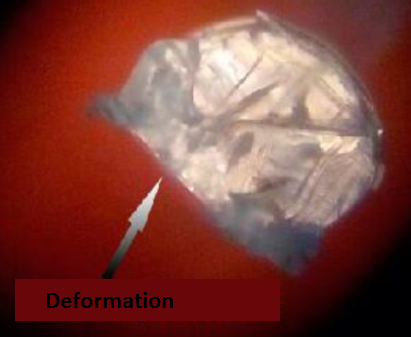
\includegraphics[width=\textwidth]{4ResearchAndDevelopments/41Fibers/DeformationFiberEnds.png}  
    \caption{\label{subfig:FiberEndDeformation}}
    \end{subfigure}
    \hfill
    \begin{subfigure}[b]{0.45\textwidth}
    \centering
    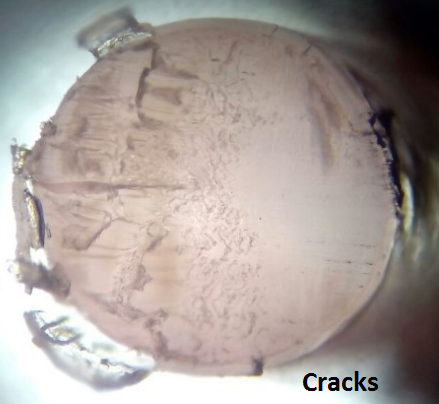
\includegraphics[width=\textwidth]{4ResearchAndDevelopments/41Fibers/CracksEndFibers.png}  
    \caption{\label{subfig:FiberEndCracks}}
    \end{subfigure}
 \caption{Unsuccessful results of using commercial techniques to cleave fibers a) Fiber end deformation b) Fiber end cracks.}
 \label{fig:BadCleavesOfFibers}
\end{figure}

The microscope model PB 4161 from EUROMEX and the Digital Microscope from Jiusion were used to check the results in the fiber ends. 

Because commercial devices do not work for our scintillating fibers, a cleaving device, shown in Figure \ref{fig:CleaveTRITIUMDevice}, was designed, built and tested.

\begin{figure}[hbtp]
\centering
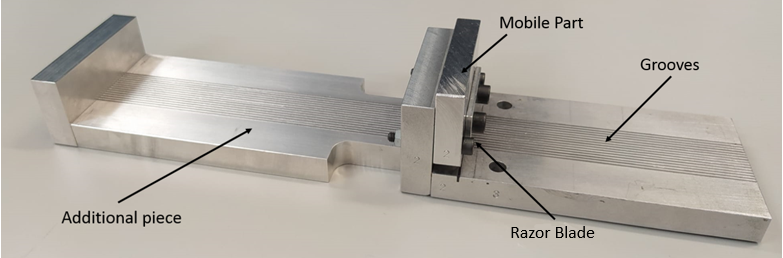
\includegraphics[scale=0.4]{4ResearchAndDevelopments/41Fibers/CuttingDevice.png}
\caption{Cleaving device. \label{fig:CleaveTRITIUMDevice}}
\end{figure}

This device consists of fourteen grooves to which fibers are hold and a thin blade, attached to a mobile piece, which is used to cleave them. The perpendicular cleave, which is one of the requirements, can be ensured since the moving piece, to which the blade is attached, is set perpendicular to the fibers. The blade used is a typical commercial razor blade, of $0.1~\mm$ thickness, which is the thickness that gave the best results. The blade was adjusted with $5\degree$ tilt, with respect to the horizontal axis since it was found in several studies that this helps to obtain a less aggressive and cleaner cleave \cite{AngleBlade, TemperatureBlade}. As it can be seen in Figure \ref{subfig:CleaveFiberEnd}, with this cleaving device fiber ends without breaks or deformation were obtained. An additional parameter that could in principle affect the cleaving quality of the fiber ends is the temperature of both, fiber and blade. A study was carried out in which both were subject to different temperatures from room temperature to 110 degrees. No significant conclusions were obtained \cite{TFGAlberto}. Thus, the cleaving process was carried out at room temperature to make the cleaving process easier.

To set the fiber length, which is the last requirement, an additional piece was designed and built, shown in Figure \ref{fig:CleaveTRITIUMDevice}. With the help of this piece, an uncertainty of less than 1 millimeter in the fiber length was achieved. With this cleaving device all the requirements imposed were fulfilled, obtaining fibers with optimal light transmission. The quality fiber end after cleaving is shown in Figure \ref{subfig:CleaveFiberEnd}. The slightly darkened zone at the bottom of the fiber is an inavoidable effect of the cleaving process and, to reduce this effect, a polishing process developed by Thorlabs was applied \cite{DiamondThorlabs}. It consists on rubbing the fibbers during two minuts with five different polishing papers, with a decreasing grain size, $30~\mu\meter$, $20~\mu\meter$, $12~\mu\meter$, $5~\mu\meter$ and $0.3~\mu\meter$, describing on the the paper a shape of an 8 (approximately 120 movements). The result obtained after polishing is shown in Figure \ref{subfig:PolishFiberEnd}, where it can be noted that the darkened zone has completely disappeared and the fiber end is completely clear without any damage or imperfection. Therefore, both tasks, cleaving and polishing,  are necessary.

\begin{figure}
\centering
    \begin{subfigure}[b]{0.5\textwidth}
    \centering
    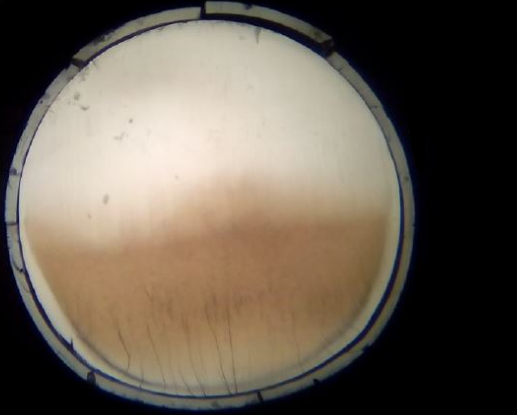
\includegraphics[width=\textwidth]{4ResearchAndDevelopments/41Fibers/CutEndFiberGood.png}  
    \caption{\label{subfig:CleaveFiberEnd}}
    \end{subfigure}
    \hfill
    \begin{subfigure}[b]{0.45\textwidth}
    \centering
    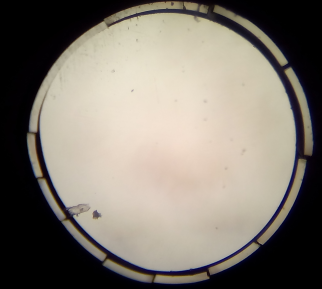
\includegraphics[width=\textwidth]{4ResearchAndDevelopments/41Fibers/CutAndPolishedFiberEnd.png}  
    \caption{\label{subfig:PolishFiberEnd}}
    \end{subfigure}
 \caption{Result of the polishing process. a) Fiber end after cleaving b) Fiber end after cleaving and polishing with Thorlabs technique.}
 \label{fig:ResultofPolishingProcess}
\end{figure}